\documentclass{article}
\usepackage[utf8]{inputenc}
\usepackage{amsmath} 
\usepackage{graphicx}
\usepackage{fancyhdr} 
\usepackage{enumitem}
\usepackage{hyperref}
\usepackage{url}
\usepackage{float}
\usepackage{amssymb}

\usepackage[backend=biber, style=ieee]{biblatex}
\addbibresource{bibliografia.bib}



\title{Trabajo 1 - Ecuaciones}
\author{FABIO ANDRES GARCIA PEREZ}
\date{Abril 2025}

\begin{document}

\maketitle

\section*{Introducción}

En este trabajo se estudiarán las ecuaciones diferenciales de primer orden, poniendo en práctica tanto el desarrollo teórico como su aplicación en situaciones concretas. Se abordarán los métodos para obtener soluciones generales y particulares, así como la interpretación gráfica de estas a través de mapas de pendientes.

El trabajo se divide en dos partes principales. La primera parte se enfoca en el análisis y solución de una ecuación diferencial de primer orden. La segunda parte plantea un problema aplicativo, el cual será modelado y resuelto mediante herramientas propias del cálculo diferencial.

\section{Primera parte: Ecuación diferencial de primer orden}

En esta sección se trabajará con la siguiente ecuación diferencial de primer orden:

\[
2y + 7\frac{dy}{dx} = \frac{5}{y}
\]

El objetivo es analizar esta ecuación, transformarla a una forma más adecuada para su resolución, y obtener su solución general. A partir de allí, se procederá con los pasos necesarios para su integración y análisis gráfico cuando sea posible.

Para la implementación de este problema, se debe tener en cuenta la condición inicial:

\[
y(0)= 14
\]

\subsection{Análisis de existencia y unicidad}

En esta etapa se determinará si la ecuación planteada posee una solución única, considerando la condición inicial y los requisitos del teorema de existencia y unicidad.

\subsubsection*{Análisis del tipo de ecuación}

La ecuación dada es:

\[
2y + 7\frac{dy}{dx} = \frac{5}{y}
\]

Esta es una ecuación diferencial de primer orden. Puede reescribirse en una forma explícita para identificar si es separable, lineal, exacta, u otra. Para ello, se despeja la derivada:

\[
\frac{dy}{dx} = \frac{1}{7} \left( \frac{5}{y} - 2y \right)
\]

\subsubsection*{Continuidad de la función}

Debemos tener en cuenta el teorema de existencia y unicidad: 

El problema de valor inicial \( \frac{dy}{dx} = f(x,y)  ; y(a) = b \) tiene al menos una solución si \( f(x,y) \) es continua en algún rectángulo R del plano XY que contiene al punto \( (a,b) \) (Esta solución existe en algún intervalo \(I\) que contiene al punto  \(x=a\)). \\
Si además se cumple que \(\frac{\partial f}{\partial y}\) también es continua, entonces la solución es única.
\vspace{0,5cm}

La expresión obtenida para \( \frac{dy}{dx} \) depende de \( y \), específicamente de funciones como \( \frac{1}{y} \) y \( y \), las cuales son continuas en su dominio. Debe evitarse \( y = 0 \), ya que genera una discontinuidad.

\subsubsection*{Continuidad de la derivada parcial respecto a \( y \)}

La derivada parcial de \( f(x, y) = \frac{1}{7} \left( \frac{5}{y} - 2y \right) \) respecto a \( y \) es:

\[
\frac{\partial f}{\partial y} = \frac{1}{7} \left( -\frac{5}{y^2} - 2 \right)
\]

Esta función también es continua en los mismos intervalos donde \( y \neq 0 \). Como tanto \( f(x, y) \) como su derivada parcial son continuas cerca del punto \( y(0) = 14 \), se garantiza la existencia y unicidad de la solución.

\subsection{Construcción del mapa de pendientes}

En esta etapa se analizará y explicará un mapa de pendientes, identificando los posibles valores de estabilización de la solución y con cuales condiciones iniciales es posible llegar a estos, adicional a esto, veremos si la ecuación diferencial  \( 2y + 7\frac{dy}{dx} = \frac{5}{y} \) es (o no) autónoma.

\subsubsection*{Mapa de pendientes}

Después de desarrollar la gráfica de pendientes utilizando Python, se obtuvo una visualización cualitativa del comportamiento de la solución. El código fuente utilizado para generar dicha gráfica puede consultarse en la bibliografía como \cite{codigo_mapaPendiente}.

\begin{figure}[H]
    \centering
    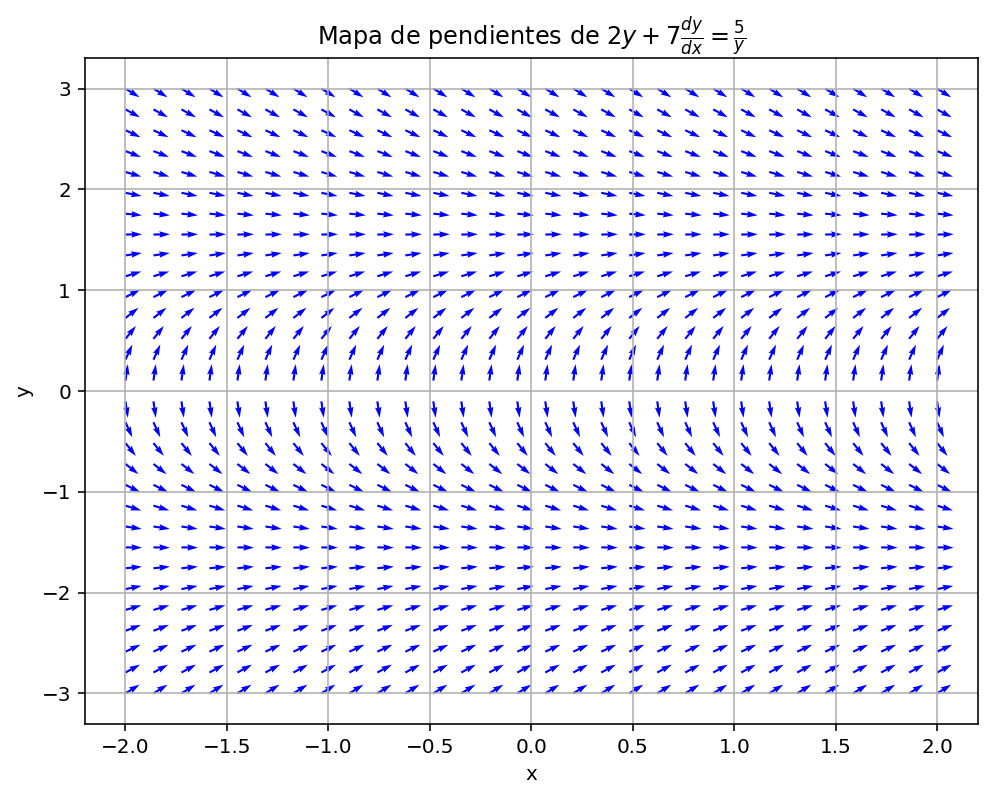
\includegraphics[width=0.7\textwidth]{MapaDePendientes.png}
    \caption{Mapa de pendientes generado en Python.}
    \label{fig:pendientes}
\end{figure}

En la figura 1 podemos observar como las flechas que representan la solución en distintos puntos muestran una clara tendencia a alejarse del eje \( y = 0 \). Esto evidencia que cerca de ese valor, el comportamiento de las soluciones cambia bruscamente, evitando que las curvas lo crucen, siendo un punto inestable, no atractor, coincidiendo con el dominio definido previamente, donde se establece que \(y \neq 0\) para garantizar la continuidad de la función y su derivada parcial. También podemos notar puntos de estabilización cerca de: \(y = -\frac{3}{2}\) y \(y = \frac{3}{2}\). Podemos ver como los valores menores a \(y = -\frac{3}{2}\) suben hasta estabilizarse en ese punto (teniendo en cuenta que estos valores de estabilización solo son aproximados), entre 0 y \(y = -\frac{3}{2}\) bajan hasta estabilizarse en ese ultimo punto, y los superiores a 0 se estabilizan cerca de \(y = \frac{3}{2}\), por ultimo, los valores superiores a \(y = \frac{3}{2}\), tienen a bajar hasta estabilizarse en \(y = \frac{3}{2}\).

\begin{figure}[H]
    \centering
    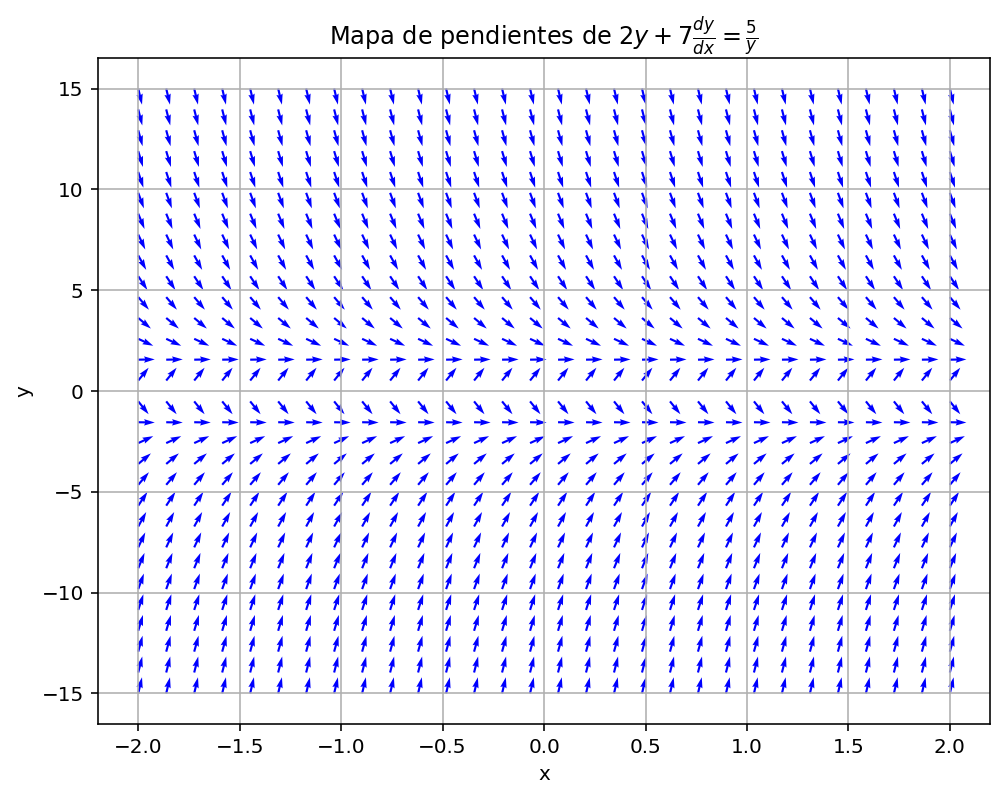
\includegraphics[width=0.7\textwidth]{MapaDePendientes2.png}
    \caption{Mapa de pendientes incluyendo valor inicial \( y(0) = 14 \).}
    \label{fig:pendientes2}
\end{figure}

Ahora, en la figura 2 podemos observar que el punto del valor inicial, también tiende al punto de estabilización en aproximadamente \(y = \frac{3}{2}\) pues aún no hemos calculado el valor exacto. Para esto podemos analizar los puntos de equilibro, al igualar la ecuación \( \frac{dy}{dx}= f(y) \) teniendo \(f(y)\) solo en términos de \(y\). Sabemos que esto se cumple en nuestra EDO, puesto que lo hicimos anteriormente:

\[
\frac{dy}{dx} = \frac{1}{7} \left( \frac{5}{y} - 2y \right)
\]
Por lo que tenemos una EDO autónoma, pues la variable independiente (\(x\)) no aparece de forma explicita en la ecuación. \\ 
Gracias a que tenemos una EDO autónoma podemos buscar los puntos de estabilización encontrando los puntos críticos, donde \(\frac{dy}{dx}=0\).\\

Encontrando los valores de (\(y\)):

\[
7\left(\frac{1}{7} \left( \frac{5}{y} - 2y \right) = 0\right)
\]

Multiplicamos por \(y\) suponiendo \(y \neq 0\).

\[
y\left(\left( \frac{5}{y} - 2y \right) = 0\right)
\]

Restamos 5 a toda la igualdad.

\[
 (5 - 2y^2)-5  = (0)-5
\] \\ 

Multiplicamos por \(-\frac{1}{2}\).

\[
 -\frac{1}{2}\left((- 2y^2)  = -5\right)
\]

Sacamos en ambos lados de la igualdad.

\[
 \sqrt{(y^2)}=\sqrt{(\frac{5}{2})}
\]

Lo que nos daría:

\[
 y=\pm\sqrt{\frac{5}{2}}
\]
Así que los valores de estabilización son \(y=\sqrt{\frac{5}{2}}\) y \(y=-\sqrt{\frac{5}{2}}\), que son \(y\approx1.58\) y \(y\approx-1.58\), lo cual coincide con los valores aproximados obtenidos con la gráfica de la figura 1. También podemos notar como al evaluar algún punto, se puede confirmar lo dicho en la descripción de la figura 1, encontrando los intervalos adecuados, por ejemplo, si elegimos un valor mayor al punto \(y=\sqrt{\frac{5}{2}}\), su \(\frac{dy}{dx}\) debería ser menor que 0, siendo una pendiente que va hacia abajo, al igual que se ve en la gráfica de la figura 2.

Si \(y=14\):

\[
 \frac{dy}{dx}=\frac{1}{7}\left(\frac{5}{y}-2y\right)=\frac{1}{7}\left(\frac{5}{14}-2(14)\right)\approx-3.94
\]

\[
 \Rightarrow \frac{dy}{dx}<0
\]

\subsection{Solución de la EDO}

En esta parte encontraremos una función \(y(x)\) que satisfaga la ecuación dada con su valor inicial, para esto usaremos el método de solución separable:

\[
 \frac{dy}{dx} = \frac{1}{7} \left( \frac{5}{y} - 2y \right)
\]

Dividimos ambos lados de la igualdad por \(\frac{5}{y}-2y\).

\[
 \frac{dy}{(dx)(\frac{5}{y}-2y)}=\frac{1}{7}
\]

Multiplicamos ambos lados por \(dx\).

\[
 \frac{1}{\frac{5}{y}-2y}dy=\frac{1}{7}dx
\]

Simplificando esta expresión \(\frac{5}{y}-2y\), para poder restar esto, multiplicamos por \("1"\) a \(2y\), pero ese \("1"\) lo podemos escribir como \(\frac{y}{y}\), lo que nos daría \(\frac{2y^2}{y}\), y remplazando esto en la expresión original, tendríamos como resultado \(\frac{5-2y^2}{y}\), por lo que en nuestra ecuación tendríamos \(\frac{1}{\frac{5-2y^2}{y}}\) que se puede reescribir como \(\frac{y}{5-2y^2}\), quedándonos con esto:

\[
 \frac{y}{5-2y^2}dy=\frac{1}{7}dx
\]

integramos ambos lados.

\[
 \int\frac{y}{5-2y^2}dy=\int\frac{1}{7}dx
\]

Resolviendo la integral de la derecha simplemente seria \(\frac{1}{7}\int dx\) lo que nos da \(\frac{1}{7}x+C\) o \(\frac{x}{7}+C\). Para resolver la integral de la izquierda, debemos emplear el método de sustitución, pues vemos que en el numerador tenemos, en parte, la derivada del denominador.

\[
 u=5-2y^2\quad,\quad du=-4y\,dy\Rightarrow-\frac{1}{4}du=y\,dy
\]

Reemplazando y reorganizando la expresión original \(\int\frac{y}{5-2y^2}dy\).

\[
 -\frac{1}{4}\int \frac{1}{u}du=-\frac{1}{4}ln|u|+C 
\]

Ahora volvemos a remplazar  \(u=5-2y^2\) para regresar a la variable original: \(-\frac{1}{4}ln|5-2y^2|+C\), por lo que del resultado de las integrales tendríamos: 

\[
 -\frac{1}{4}ln|5-2y^2|+C=\frac{x}{7}+C
\]

Sumamos ambas constantes, pues esto nos daría otra constante, la cual expresaremos como \(C_2\), quedándonos \(-\frac{1}{4}ln|5-2y^2|=\frac{x}{7}+C_2\) además de esto, sabemos que \(e^u=e^v\) siempre y cuando \(u=v\), por lo que diremos que \(u=-\frac{1}{4}ln|5-2y^2|\) y \(v=\frac{x}{7}+C_2\), dando como resultado: 

\[
 e^{-\frac{1}{4}ln|5-2y^2|}=e^{\frac{x}{7}+C_2}
\]

Por propiedades de los logaritmos, sabemos que \(k\cdot ln|a|=ln|a^k|\), por lo que \(-\frac{1}{4}ln|5-2y^2|=ln|(5-2y^2)^{-\frac{1}{4}}|\), reemplazando esto en la ecuación anterior: 

\[
 e^{ln|(5-2y^2)^{-\frac{1}{4}}|}=e^{\frac{x}{7}+C_2}
\]

Dado que \(e^k\) y \(ln(k)\) son funciones inversas, se cumple que \(e^{ln(k)}=k\) para todo \(k>0\), también por propiedades de los exponentes, \(x^{u+v}=x^u\cdot x^v\), con esto en cuenta, podemos simplificar aún más la ecuación:

\[
 (5-2y^2)^{-\frac{1}{4}}=e^{\frac{x}{7}}\cdot e^{C_2}
\]

Euler elevado a una constante arbitraria, dará como resultado otra constante arbitraria, la cual podemos establecer como \(C_3\), adicional a esto simplificamos el exponente negativo del lado izquierdo.

\[
 \frac{1}{(5-2y^2)^{\frac{1}{4}}}=C_3\cdot e^{\frac{x}{7}}
\]

Multiplicando toda la igualdad por \(\frac{(5-2y^2)^{\frac{1}{4}}}{C_3\cdot e^{\frac{x}{7}}}\).

\[
 \frac{1}{C_3\cdot e^{\frac{x}{7}}}= (5-2y^2)^{\frac{1}{4}}
\]

Elevando ambos lados a la 4.

\[
 \frac{1}{(C_3\cdot e^{\frac{x}{7}})^{4}}=5-2y^2
\]

Restamos 5 en ambos lados.

\[
 \frac{1}{(C_3\cdot e^{\frac{x}{7}})^{4}}-5=-2y^2
\]

Multiplicamos por \(-\frac{1}{2}\)

\[
 -\frac{1}{2(C_3\cdot e^{\frac{x}{7}})^{4}}+\frac{5}{2}=y^2
\]

Por propiedad de los exponentes tenemos que \((ab)^n=a^n\cdot b^n\), entonces \((C_3\cdot e^{\frac{x}{7}})^{4}=C_3^4\cdot e^{\frac{4\cdot x}{7}}\). Podemos escribir una constante \(C_3^4\) como otra constante arbitraria, \(C_4\), adicional a esto podemos expresar \(\frac{1}{C_4\cdot e^{\frac{4\cdot x}{7}}}\) como \(C_4\cdot e^{-\frac{4\cdot x}{7}}\) por lo que nos quedará \(\frac{-C_4\cdot e^{-\frac{4\cdot x}{7}}}{2}+\frac{5}{2}=y^2\).

Simplificamos la suma, y teniendo en cuenta lo anterior sobre constantes arbitrarias, podemos escribir \(-C_4\) como \(C_5\).

\[
 \frac{C_5\cdot e^{-\frac{4\cdot x}{7}}+5}{2}=y^2
\]

Despejando '\(y\)':

\[
 y =\pm\sqrt{\frac{C_5\cdot e^{-\frac{4\cdot x}{7}}+5}{2}}
\]

Sabemos que \(y\) es función de \(x\), así que escribiendo nuestra solución de la EDO de manera formal, tendremos la siguiente solución general:

\[
 y(x) =\pm\sqrt{\frac{C_5\cdot e^{-\frac{4\cdot x}{7}}+5}{2}}
\]

Esta es la solución general de la ecuación diferencial. Sin embargo, al evaluar la condición inicial \(y(0) = 14\), y dado que \(14 > 0\), tomaremos únicamente la rama positiva de la raíz cuadrada. Por tanto, la solución particular será:

\[
 y(x) = \sqrt{\frac{C_5\cdot e^{-\frac{4\cdot x}{7}}+5}{2}}
\]

Reemplazando \(y(0)=14\)

\[
 14=\sqrt{\frac{C_5\cdot e^{-\frac{4(0)}{7}}+5}{2}}
\] 

Elevamos ambos lados a la 2, y realizamos el producto de \(-\frac{4(0)}{7}=0\).

\[
 196=\frac{C_5\cdot e^{0}+5}{2}
\] 

Multiplicamos por 2 toda la igualdad, y al tener un numero con potencia de 0, este número seria igual a 1.

\[
 392=C_5+5
\] 

Restamos 5 en ambos lados de la igualdad

\[
 387=C_5
\]

Regresando a la expresión \(y(x) = \sqrt{\frac{C_5\cdot e^{-\frac{4\cdot x}{7}}+5}{2}}\) y reemplazando el valor de \(C_5\) obtenemos nuestra solución particular:

\[
 y(x) = \sqrt{\frac{387\cdot e^{-\frac{4\cdot x}{7}}+5}{2}}
\]
Si reescribimos la expresión de la solución general como \(y(x)=\sqrt{\frac{C_5}{2}e^{-\frac{4\cdot x}{7}}+\frac{5}{2}}\), podemos observar que si \(x \to \infty\), la expresión \(\frac{C_5}{2}e^{-\frac{4\cdot x}{7}}\) va a tender a ser 0, lo que nos dejaría que si \(x \to \infty\), \(y(x\to \infty)=\pm\sqrt{\frac{5}{2}}\), cumpliendo con los puntos de estabilización anteriormente encontrados. También podemos notar que el intervalo de validez sera \(\forall x \in \mathbb{R}\), pero esto también nos cumple el intervalo de existencia y unicidad, ya que '\( e^{-\frac{4\cdot x}{7}}\)' siempre será un valor positivo, sin importar cuanto valga \(x\), haciendo que dentro de la raíz siempre haya un valor mayor a 0, por lo que se cumple que \(y\neq0\). 

\subsection{Solución de la EDO usando Sympy}

Acá veremos la solución general y la solución particular con el problema de valor inicial, usando el paquete sympy de python, comparemos estas soluciones inmediatas con las realizadas paso a paso durante la solución de la EDO, el código fuente de esta solución se puede consultar en la bibliografía como \cite{codigo_mapaPendiente}.

Al ejecutar el archivo .py, obtenemos en la consola dos funciones diferentes\(y(x)=g(x)\), que hacen referencia a la solución general, y otra función que hace referencia a la solución particular, las cuales serian:

Para la solución general:
\begin{align*}
y(x)&=\frac{-\sqrt{2}\cdot\sqrt{C_1\cdot e^{\frac{-4\cdot x}{7}}+5}}{2} \\
y(x)&=\frac{\sqrt{2}\cdot\sqrt{C_1\cdot e^{\frac{-4\cdot x}{7}}+5}}{2} 
\end{align*}

Para la solución particular:
\[
 y(x)=\frac{\sqrt{2}\cdot\sqrt{5+387\cdot e^{\frac{-4\cdot x}{7}}}}{2}
\]
Las expresiones para la solución general se pueden reescribir como:

\[
 y(x)=\pm\frac{\sqrt{2}\cdot\sqrt{C_1\cdot e^{\frac{-4\cdot x}{7}}+5}}{2} 
\]
nuestra expresión general es \(y(x) =\pm\sqrt{\frac{C_5\cdot e^{-\frac{4\cdot x}{7}}+5}{2}}\), por lo que se debe cumplir la siguiente igualdad:

\[
 \pm\frac{\sqrt{2}\cdot\sqrt{C_1\cdot e^{\frac{-4\cdot x}{7}}+5}}{2}=\pm\sqrt{\frac{C_5\cdot e^{-\frac{4\cdot x}{7}}+5}{2}}
\]

Se puede obtener la solución general obtenida en sympy usando un poco de álgebra sobre nuestra solución general, para esto lo primero que haremos es recurrir de nuevo a multiplicar por 1, o en este caso, por \(\frac{2}{2}\), esto lo pondremos dentro de la raíz, lo cual realmente no alterará nada, pues como se explicó anteriormente, es lo mismo que multiplicar por 1, y \(a\cdot1=a\).

\[
 y(x) =\pm\sqrt{\frac{2}{2}\cdot\frac{C_5\cdot e^{-\frac{4\cdot x}{7}}+5}{2}}
\]

Al realizar el producto en el denominador obtenemos:

\[
 y(x) =\pm\sqrt{\frac{2(C_5\cdot e^{-\frac{4\cdot x}{7}}+5)}{4}}
\]

Por propiedades matemáticas sabemos lo siguiente: \(\sqrt{ab}=\sqrt{a}\cdot\sqrt{b}\) y \(\sqrt{\frac{a}{b}}=\frac{\sqrt{a}}{\sqrt{b}}\) por lo que podemos reescribir la expresión anterior como:

\[
 y(x) =\pm\sqrt{2}\frac{\sqrt{C_5\cdot e^{-\frac{4\cdot x}{7}}+5}}{\sqrt{4}}
\]

Resolviendo \(\sqrt{4}=2\) obtenemos en nuestra solución general \(y(x) =\pm\sqrt{2}\frac{\sqrt{C_5\cdot e^{-\frac{4\cdot x}{7}}+5}}{2}\), lo cual cumple la igualdad planteada:

\[
 \pm\frac{\sqrt{2}\cdot\sqrt{C_1\cdot e^{\frac{-4\cdot x}{7}}+5}}{2}=\pm\sqrt{2}\frac{\sqrt{C_5\cdot e^{-\frac{4\cdot x}{7}}+5}}{2}
\]

Esta igualdad se cumple, pues la única diferencia es el nombre de las constantes arbitrarias, pero como se ha dejado en claro durante el desarrollo de las soluciones, que tengan diferente nombre es lo de menos, simplemente son una constante cualquiera.
Ahora, también se debe de cumplir nuestra solución particular con la obtenida en sympy. Para esto no necesitamos realizar álgebra paso a paso, como se hizo para notar que las soluciones generales eran las mismas, con tan solo tomar nuestra ecuación general con los pequeños cambios aplicados \(y(x)=\pm\sqrt{2}\frac{\sqrt{C_5\cdot e^{-\frac{4\cdot x}{7}}+5}}{2}\), tomamos la rama positiva de esta raíz cuadrada, quedándonos con \(y(x)=\sqrt{2}\frac{\sqrt{C_5\cdot e^{-\frac{4\cdot x}{7}}+5}}{2}\), la cual, al reemplazar el valor de \(C_5\) por el valor encontrado \(C_5=387\), quedándonos \(y(x)=\sqrt{2}\frac{\sqrt{387\cdot e^{-\frac{4\cdot x}{7}}+5}}{2}\), por lo que la igualdad se debe cumplir solo con eso.

\[
 \frac{\sqrt{2}\cdot\sqrt{5+387\cdot e^{\frac{-4\cdot x}{7}}}}{2}=\sqrt{2}\frac{\sqrt{387\cdot e^{-\frac{4\cdot x}{7}}+5}}{2}
\]

Esta igualdad se cumple, pues la única diferencia es el orden en la suma, pero la suma es conmutativa, por lo que \(a+b=b+a\).
Con esto podemos notar un buen indicador de que tenemos la solución correcta, pues tanto con sympy y resolviendo paso a paso, obtuvimos el mismo resultado.

\subsection{Gráfica de la solución}

En esta ultima etapa se tendrá la gráfica la solución particular, adicional a esto, también la gráfica varios miembros de la familia de soluciones, sobrepuestas al mapa de pendientes obtenido, para esto usaremos Matplotlib, en python, código que se puede consultar en la bibliografía como \cite{codigo_mapaPendiente}.

\begin{figure}[H]
    \centering
    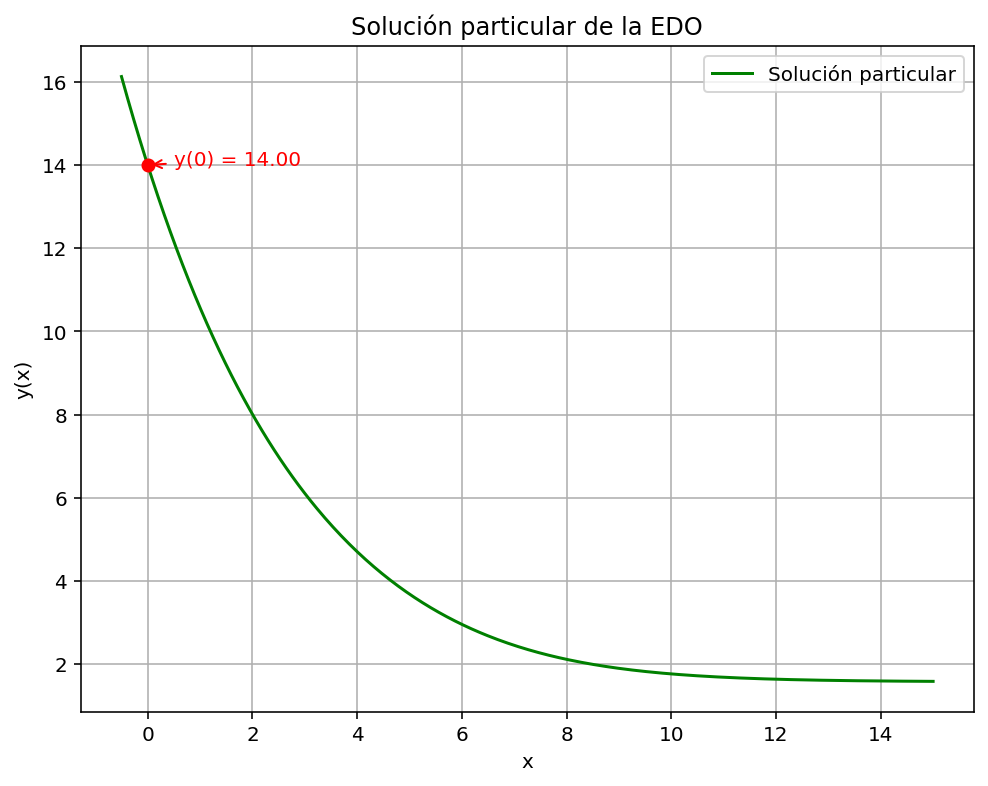
\includegraphics[width=0.7\textwidth]{Grafica_solucionP.png}
    \caption{Gráfica de la solución particular con valor inicial \( y(0) = 14 \).}
    \label{fig:sol_particular}
\end{figure}

En la figura 3 podemos ver la gráfica de nuestra solución particular, pero, ¿cómo funciona esto? Es más fácil de lo que parece, la gráfica que estamos viendo, realmente no es la gráfica "\(y(0)=14\)", es la gráfica con la constante arbitraria \(C_5=387\), en la que usando esta constante en nuestra solución, donde nos queda \(y(x) = \sqrt{\frac{387\cdot e^{-\frac{4\cdot x}{7}}+5}{2}}\), se pondrán varios puntos en la gráfica, para esto se usan las líneas \(\text{x\_vals = np.linspace(\(-0.5, 15, 400\))}\) y \(\text{y\_vals = f(x\_vals)}\), donde esos valores "\((-0.5,15,400)\)" significa el rango de valores en x, y cuantos puntos se pondrán entre ese espacio de x, separados la misma distancia, en este caso, 400 puntos entre \(-0.5\) y 15, siendo \(-0.5\) que la función comience en ese valor en x, y 15, para que termine con ese valor en x, eso mismo podemos observar en la figura 3, la posición de estos puntos en y, depende de la función, por eso no tiene un valor numérico, sino "\(\text{f(x\_vals)}\)", cada uno de estos puntos estarán conectados por una linea, de punto a punto, en orden, por ejemplo si tenemos P1,P2 y P3, ubicados en ese orden respectivamente sobre el plano, no estará conectado P1 a P3 y P2, sino P1 a P2 y P2 a P3, para poder mostrar en la gráfica una función lineal, sin cortes (a menos que esta tenga una discontinuidad), y lo más precisa posible, pues entre más valores tome, mejor se verá.

\begin{figure}[H]
    \centering
    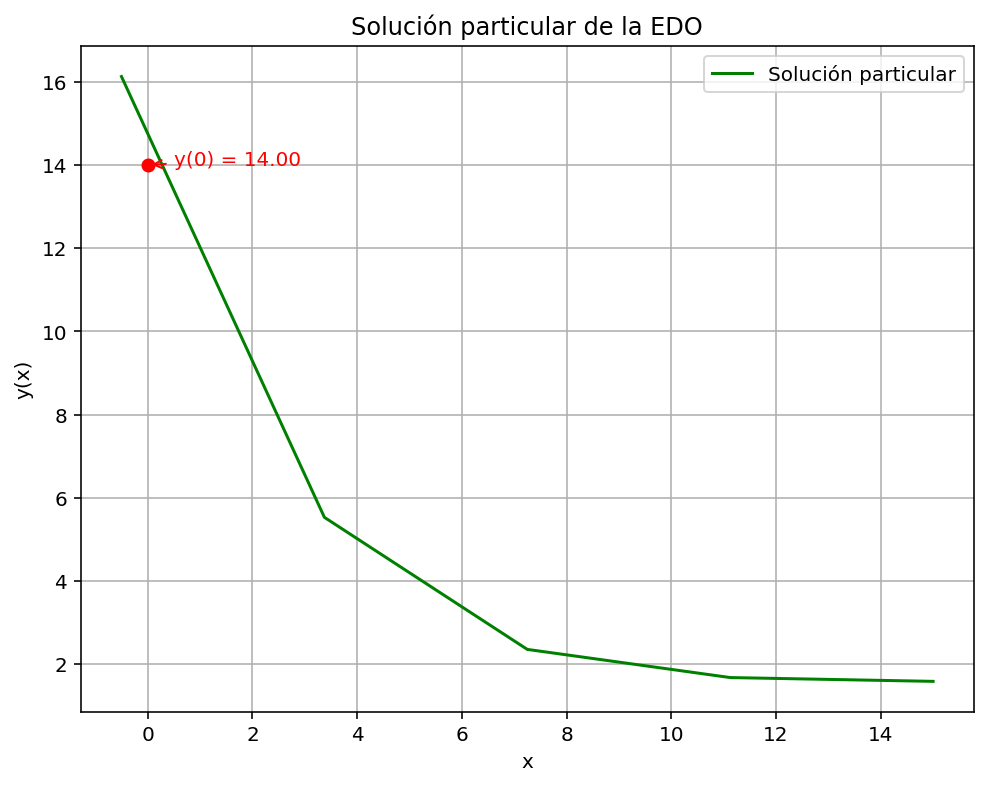
\includegraphics[width=0.7\textwidth]{Grafica_solucionP_mala.png}
    \caption{Gráfica de la solución particular con pocos puntos.}
    \label{fig:sol_particular_mala}
\end{figure}

Por ejemplo en esta figura 4 podemos notar una gráfica con solo 5 puntos, conectados por una linea (así mismo funciona la figura 3, pero con 400 puntos, haciendo esto casi imperceptible), tiene tan pocos puntos que se puede ver la falta de precisión al no tocar ni siquiera el valor inicial \(y(0)=14\). \\ \\
Volviendo a la figura 3, notamos que esta entre más aumenta su valor en \(x\), más se aproxima a \(\sqrt{\frac{5}{2}}\approx1.58\).

\begin{figure}[H]
    \centering
    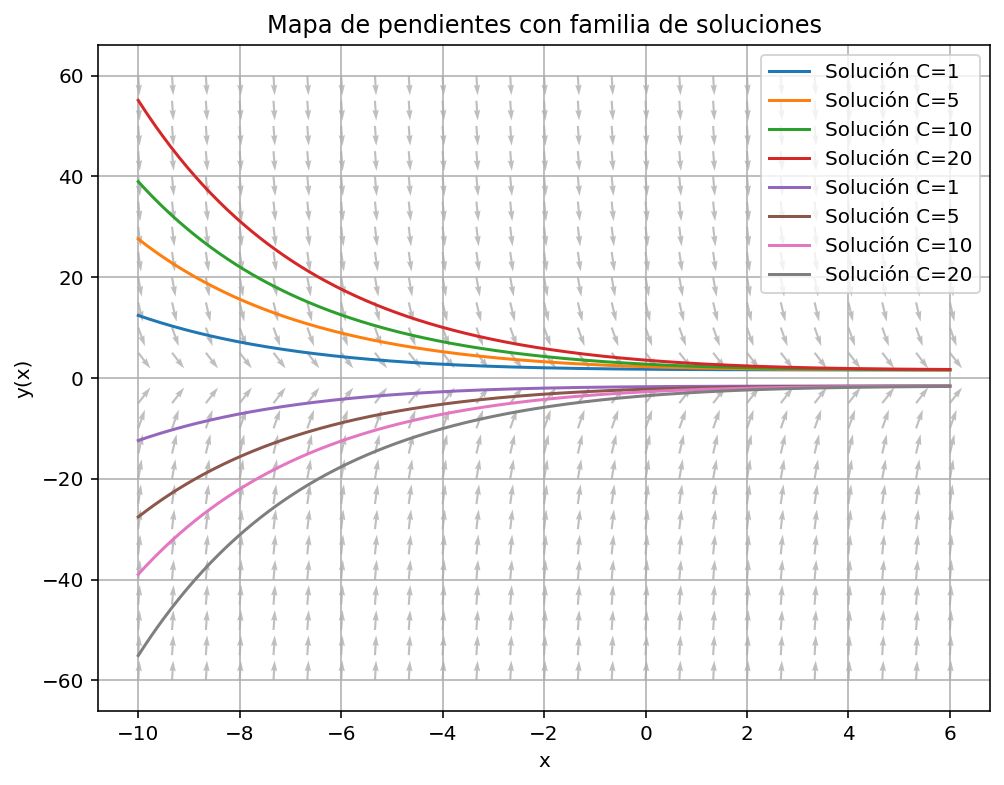
\includegraphics[width=0.7\textwidth]{Grafica_MSoluciones.png}
    \caption{Gráfica de 8 miembros de la familia de soluciones.}
    \label{fig:Familia_Soluciones}
\end{figure}

Por ultimo podemos ver en la figura 5 varias soluciones con diferentes valores para \(C_5\), los cuales están sobrepuestos a la gráfica de pendientes, pero en este caso, con diferente rango de valores (lo que no cambia en absoluto los puntos de estabilización), todas se estabilizan en el punto correspondiente, ya sea \(\sqrt{\frac{5}{2}}\) o \(-\sqrt{\frac{5}{2}}\), pero, ¿por qué están repetidos los valores de \(C_5\) y estos me dan diferentes funciones? 
Esto se da gracias a que en nuestra solución general tenemos \(\pm\sqrt{2}\frac{\sqrt{C_5\cdot e^{-\frac{4\cdot x}{7}}+5}}{2}\), así que debe haber una solución positiva y negativa, podemos escoger una en especifico según el problema de valor inicial, por ejemplo en este caso fue \(y(0)=14\), al despejar tenemos el valor de \(C_5=387\), que nos daría dos posibles opciones, una negativa y otra positiva, pero como tenemos \(y(0)=14\), significa que la función pasara por el punto \((x,y)=(0,14)\), y para que esto se cumpla, debe ser la raíz positiva, como se observa en la figura 3.

\printbibliography

\end{document}
